% !TEX program = xelatex
% !TEX encoding = UTF-8
\ifcsname wholebook\endcsname
\else
\documentclass[12pt,a4paper]{ctexbook}
% ============================================================
% 共享导言区 preamble.tex
% 本文件被 main.tex(整书编译)和各章文件(单独编译)共同引用,
% 从而保证两种编译方式下的宏包与样式完全一致。
% 注意: 本文件不含 \documentclass, 只放宏包与样式设置。
% ============================================================
\usepackage[a4paper,margin=1.1in]{geometry}
\usepackage{graphicx}
\usepackage{listings}
\usepackage{xcolor}
\usepackage[hidelinks]{hyperref}
\usepackage{tikz}
\usetikzlibrary{positioning,arrows.meta,decorations.pathreplacing,calc}
\usepackage{booktabs}

% 代码环境样式设置
\lstset{
    basicstyle=\ttfamily\small,
    keywordstyle=\color{blue}\ttfamily,
    commentstyle=\color{gray}\ttfamily,
    stringstyle=\color{red}\ttfamily,
    backgroundcolor=\color{gray!8},
    frame=single,
    rulecolor=\color{gray!40},
    breaklines=true,
    showstringspaces=false,
    columns=fullflexible,
    keepspaces=true,
    % 允许中文注释/内容正常显示
    extendedchars=true,
    literate={
        {·}{{\cdot}}1
    }
}

\begin{document}
\fi

\chapter{ROS2基础}
\section{ROS2的下载}
首先启动虚拟机中的ubuntu，打开终端，输入下面的指令。
\begin{lstlisting}[language=bash,title={一键安装指令}]
    wget http://fishros.com/install -O fishros && . fishros
\end{lstlisting}
输入密码，在选项界面选择1-一键安装ROS，接着根据你的情况选择是否更换系统源，接着等待一会就会让你选择要安装的ROS2版本了。这里选择humble版本的ROS2即可。

接着会问你安装桌面版还是基础版，我们选择桌面版，包含可视化工具，嗯，我就喜欢可视化工具，如果是在树莓派上装可以使用基础版。

安装完成后输入ros2如果看到下面的界面则安装成功。
\begin{figure}[h]
  \centering
  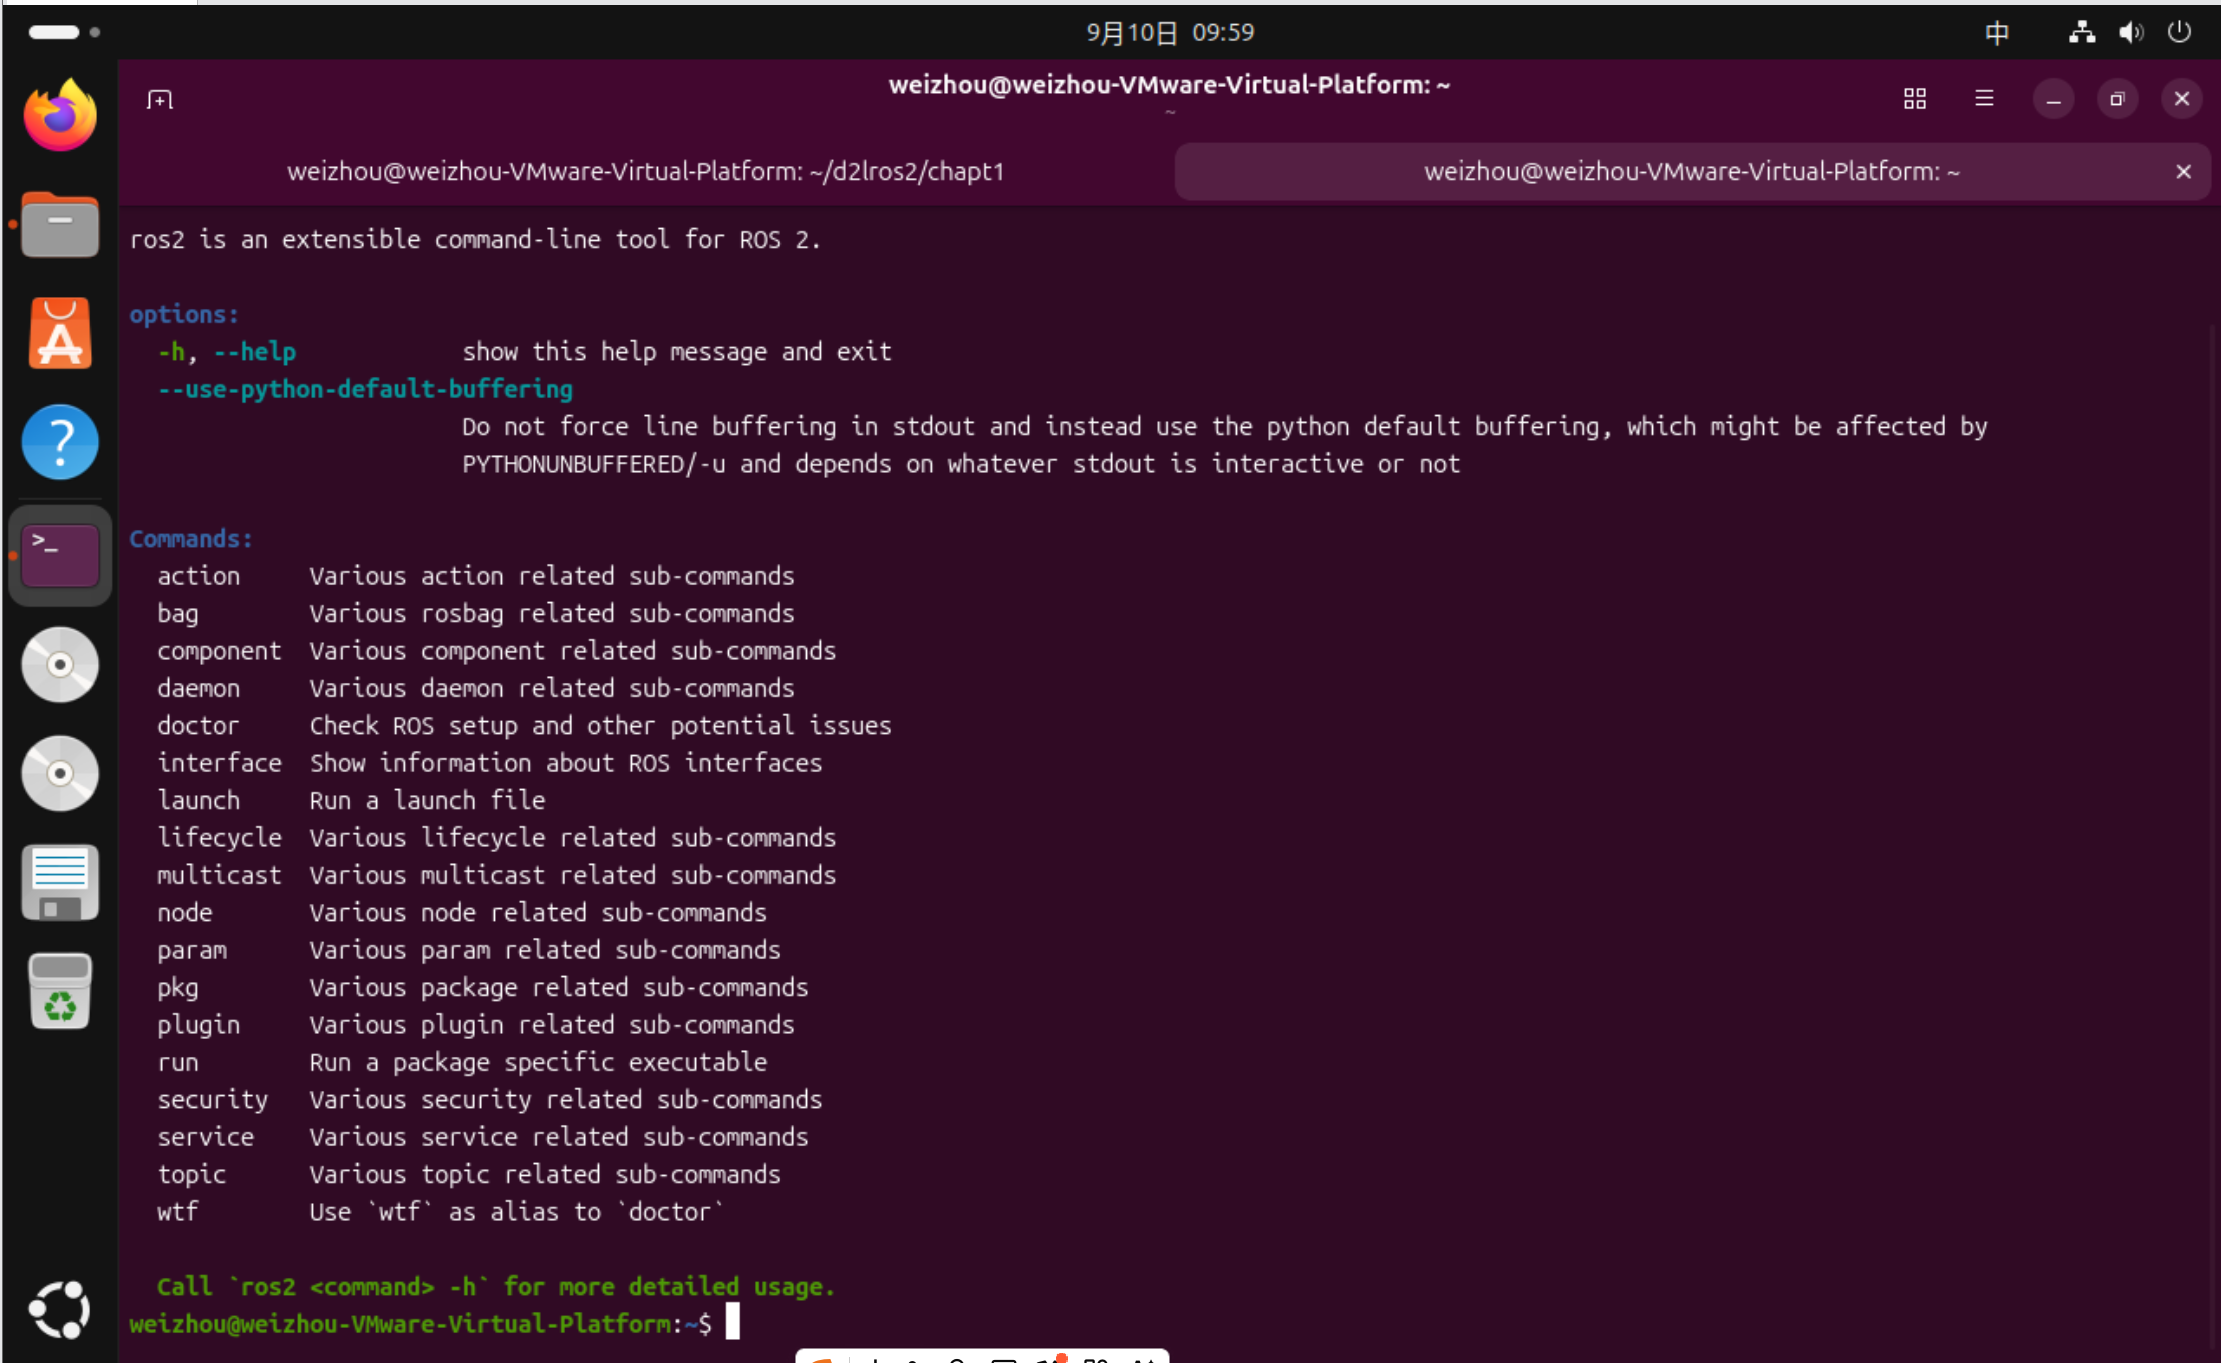
\includegraphics[width=0.8\textwidth]{Figure/ROS2成功安装界面.png}
  \caption{ROS2成功安装界面}
  \label{fig:ROS2成功安装界面}
\end{figure}

那要是我瞎玩，给ROS2环境弄乱了。该怎么办呢？删掉重装就好了呀。
\begin{lstlisting}[language=bash,title={一键卸载ROS2}]
    sudo apt remove ros-humble-*
    sudo apt autoremove
\end{lstlisting}

我们都知道安装软件要设置安装目录。那么ROS2装在哪里了呢？ROS安装的默认目录在/opt/ros/下，根据版本的名字进行区分。安装的是humble版本的ROS，所以安装目录在/opt/ros/humble下。

\section{ROS2体验}
\subsection{你说我听}
游戏内容：很简单，我们启动两个节点，一个节点负责发消息(说)，一个节点负责收消息（听）。
\begin{enumerate}
    \item 启动一个终端，快捷键 \texttt{Ctrl+Alt+T}。
    \item 在终端中启动倾听者：\verb|ros2 run demo_nodes_py listener|
    \item 再启动一个新终端，快捷键 \texttt{Ctrl+Alt+T}。
    \item 在新终端中启动说话者：\verb|ros2 run demo_nodes_cpp talker|
\end{enumerate}
观察一下现象，talker节点每数一个输，倾听节点每一次都能听到一个，是不是很神奇。
\begin{figure}[h]
  \centering
  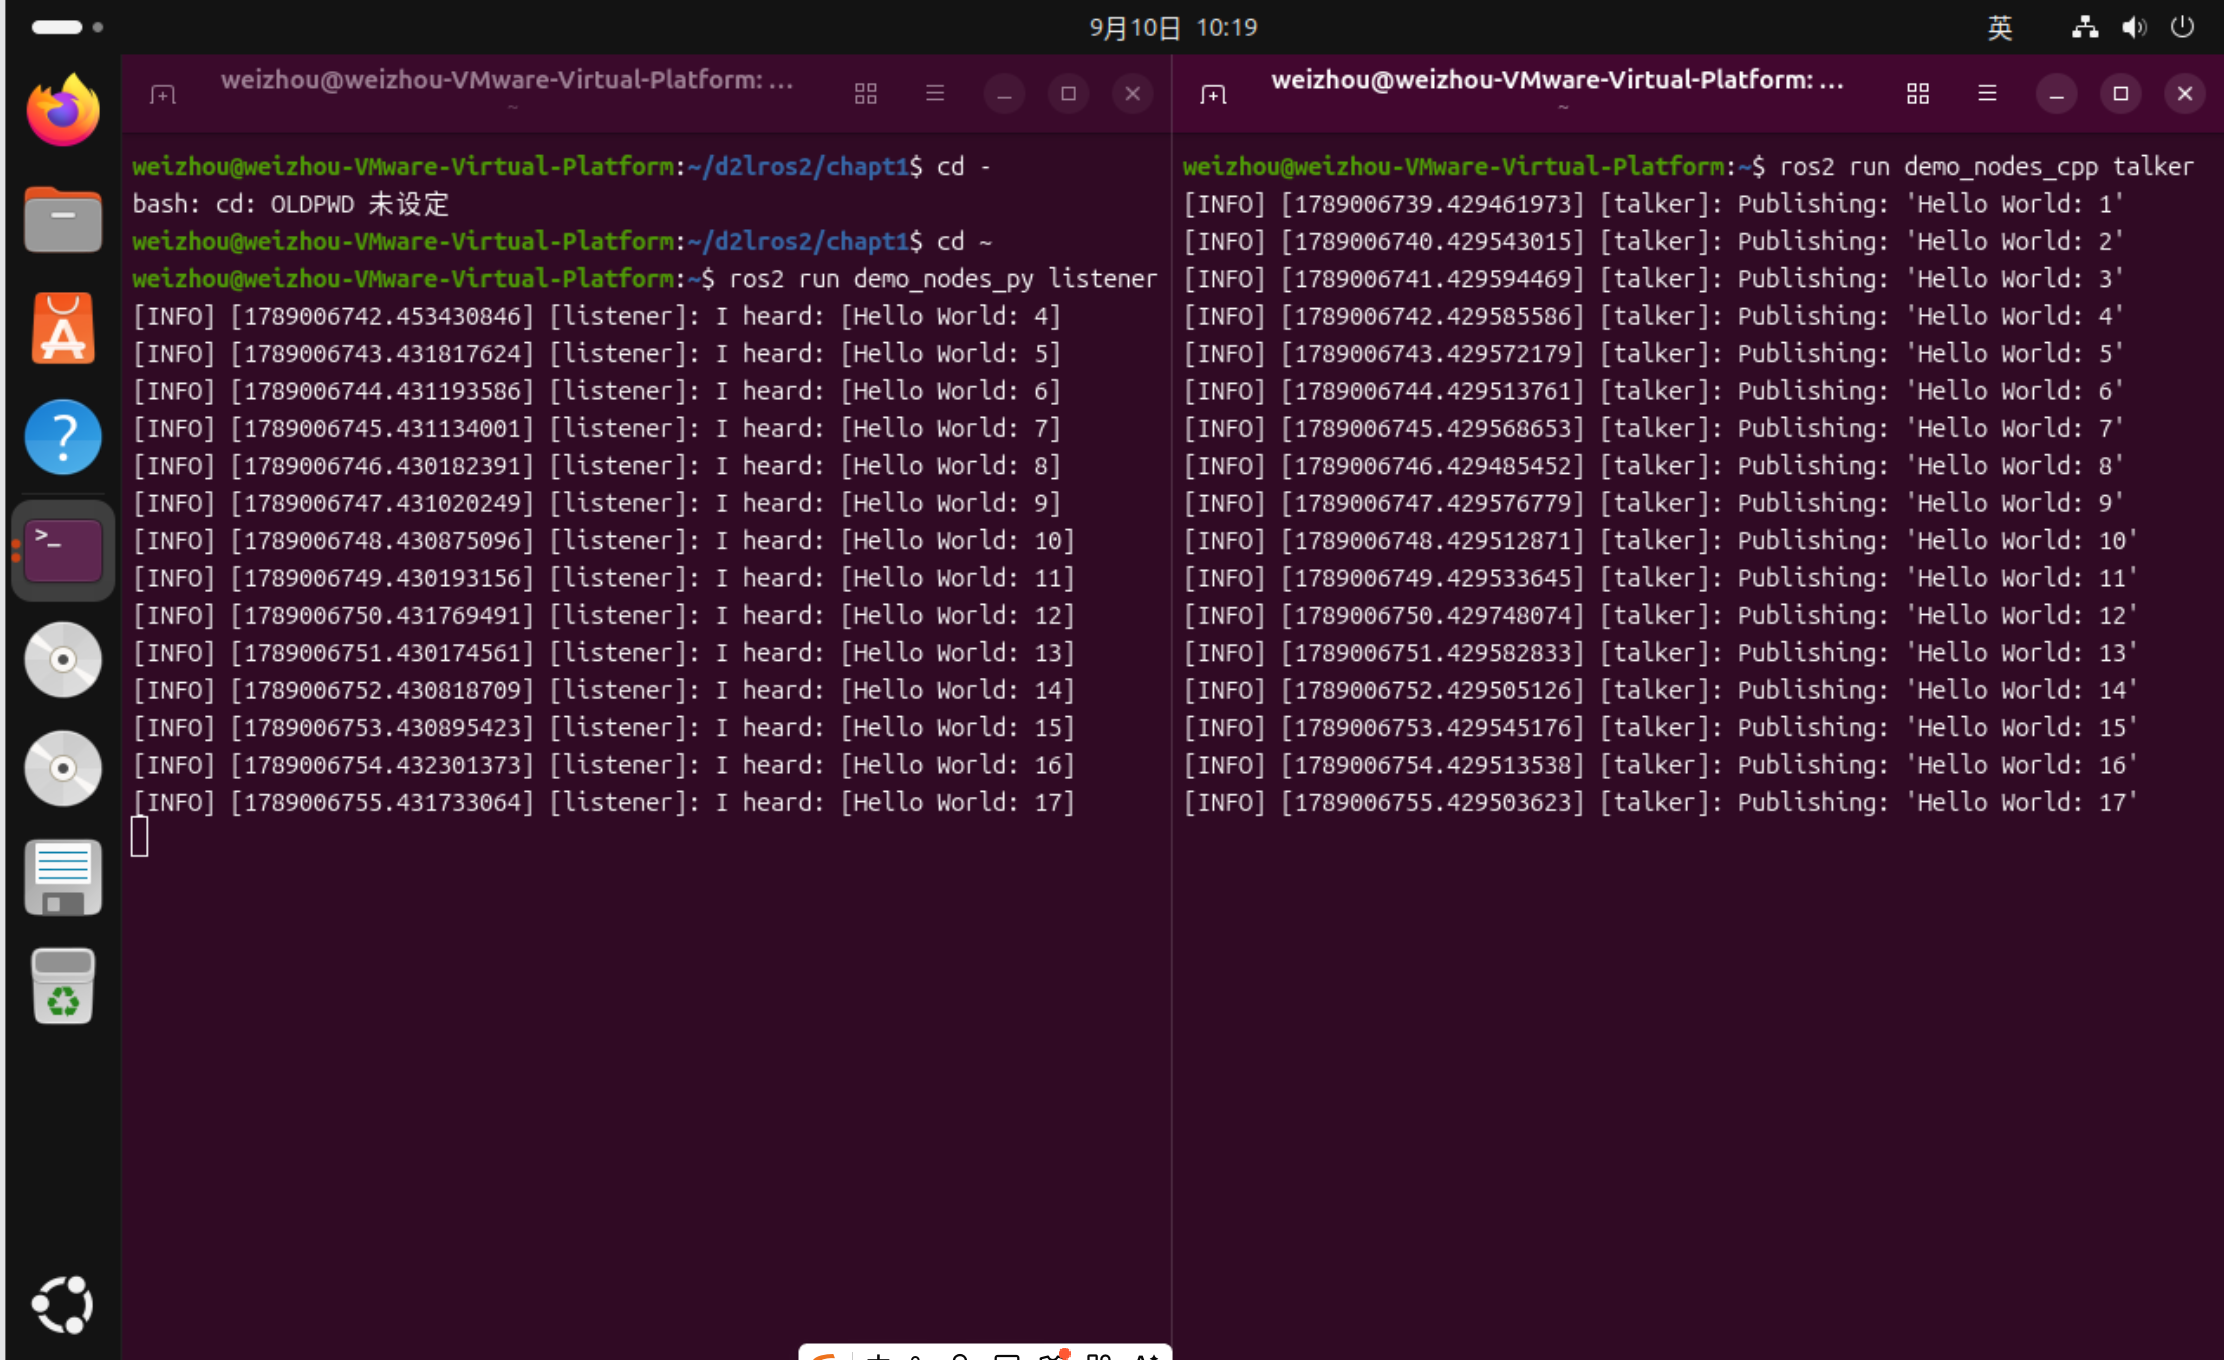
\includegraphics[width=0.8\textwidth]{Figure/你说我听.png}
  \caption{你说我听}
  \label{fig:你说我听}
\end{figure}

\subsection{涂鸦乌龟}
打开终端Ctrl+Alt+T,输入下面的指令
\begin{lstlisting}[language=bash,title={启动海龟画图}]
    ros2 run turtlesim turtlesim_node
\end{lstlisting}
如下图所示：
\begin{figure}[h]
  \centering
  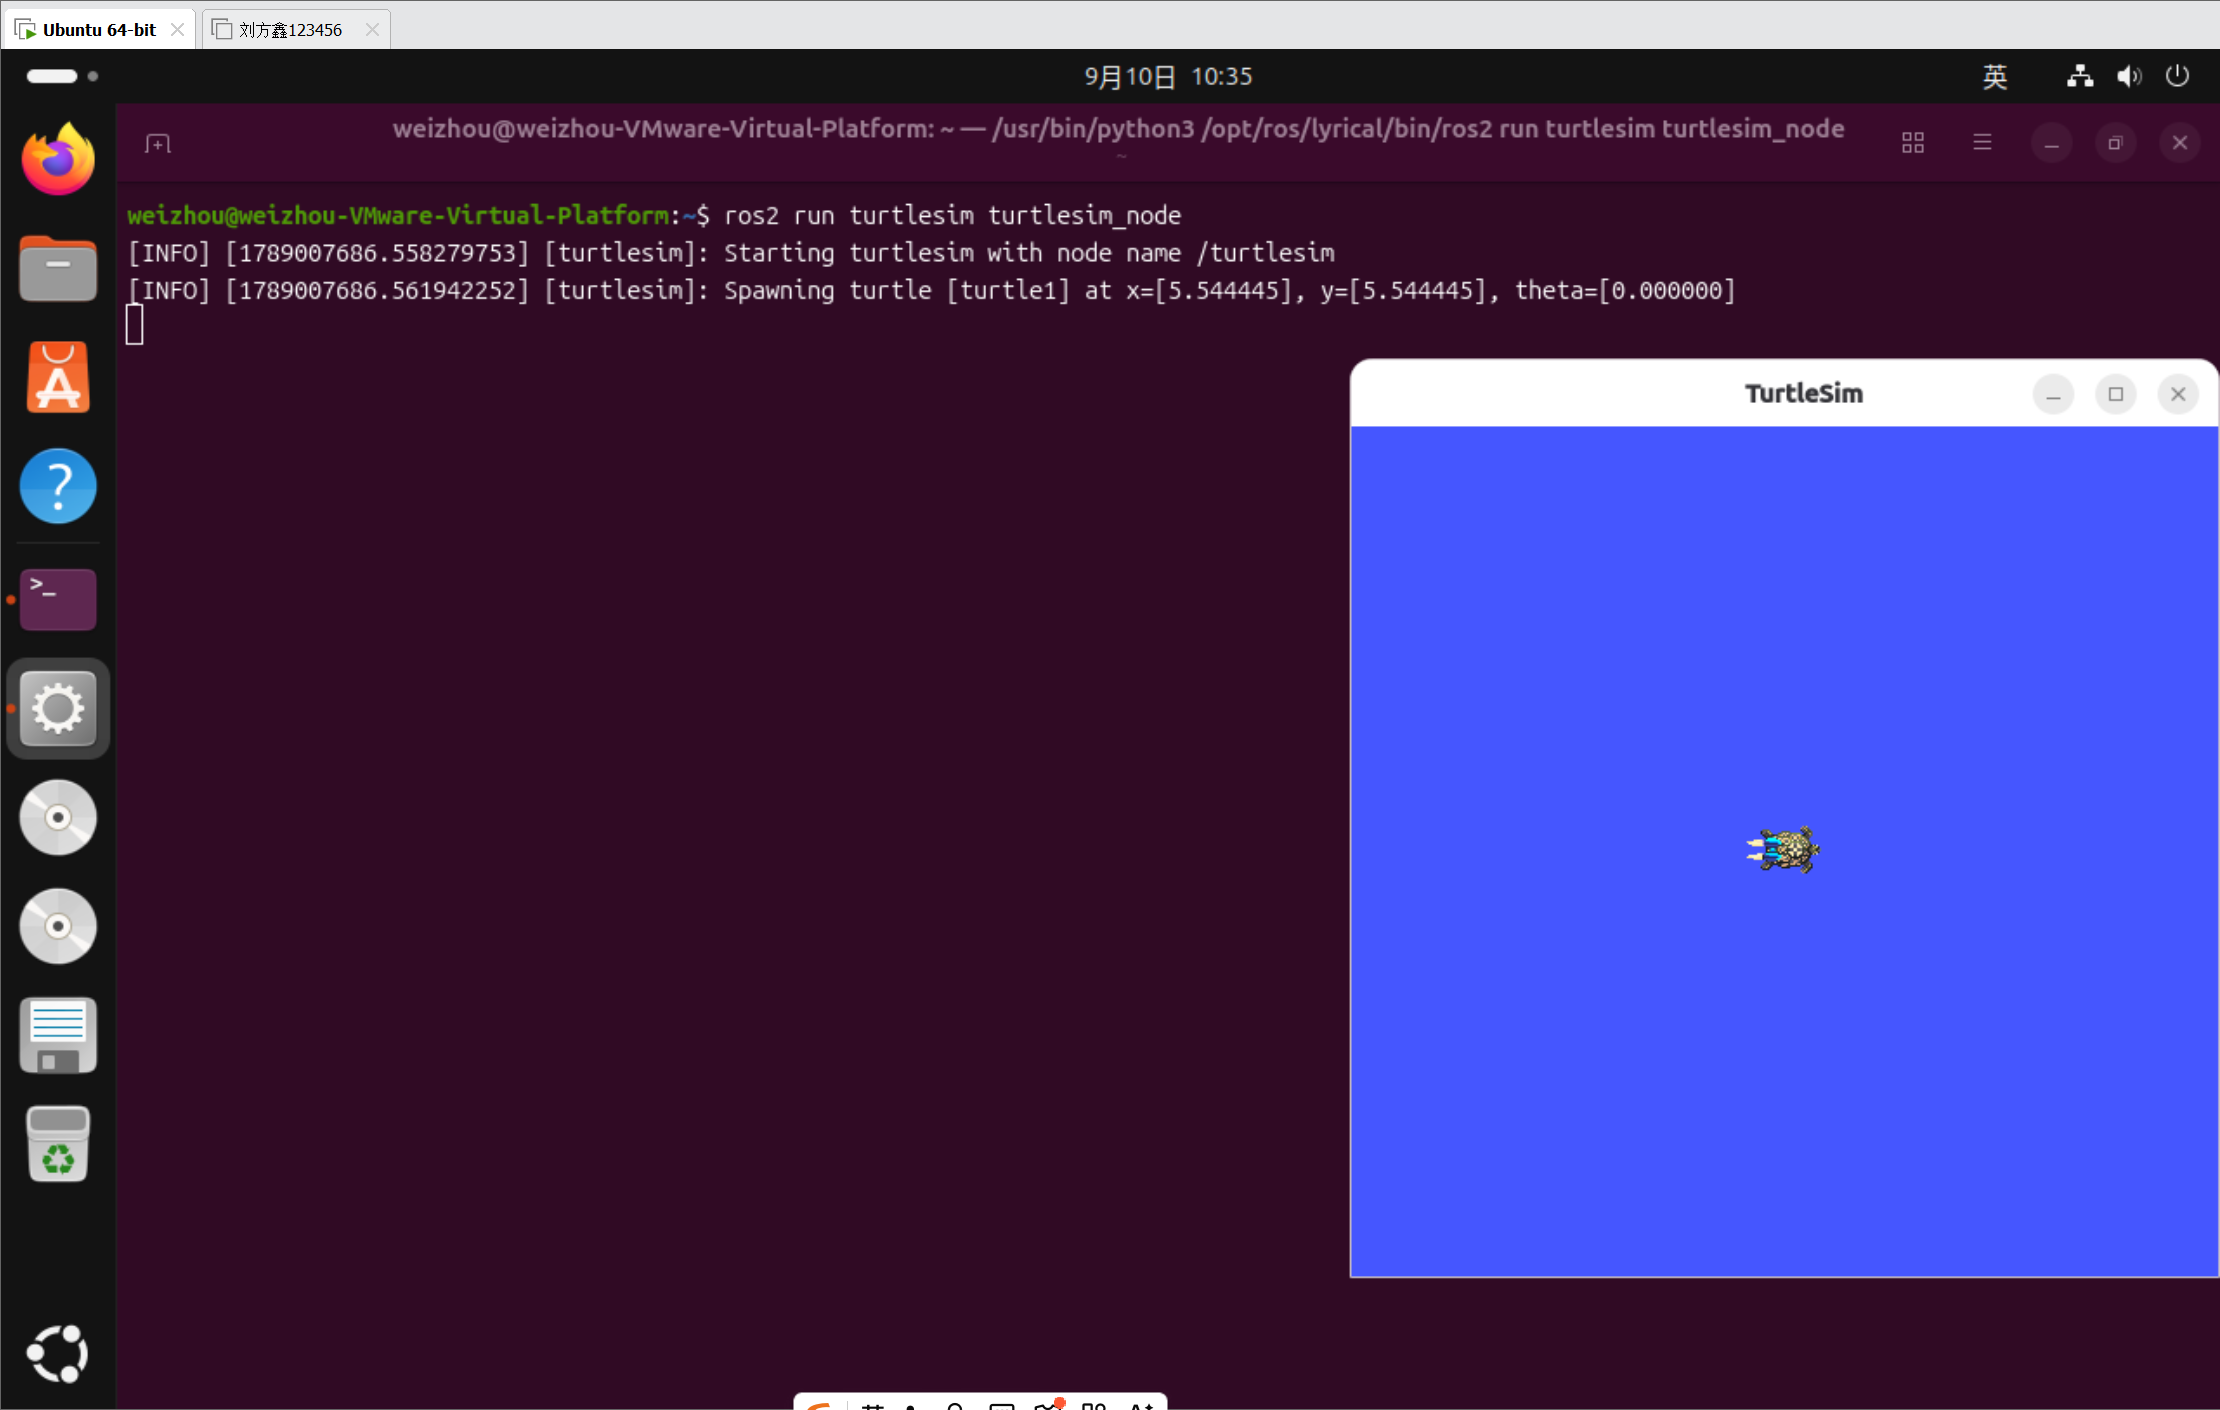
\includegraphics[width=0.8\textwidth]{Figure/海龟模拟器}
  \caption{海龟模拟器}
  \label{fig:海龟模拟器}
\end{figure}

点一下原来的终端输入Ctrl+Shift+T 打开一个新的标签页输入
\begin{lstlisting}[language=bash,title={启动海龟操控}]
    ros2 run turtlesim turtle_teleop_key
\end{lstlisting}
\newpage
\subsection{RQT可视化}
保持前面两个游戏在运行状态，打开终端，输入rqt。
打开之后选择插件Introspection / Node Graph，刷新一下，即可看见两个节点间的通信关系。
\begin{figure}[h]
  \centering
  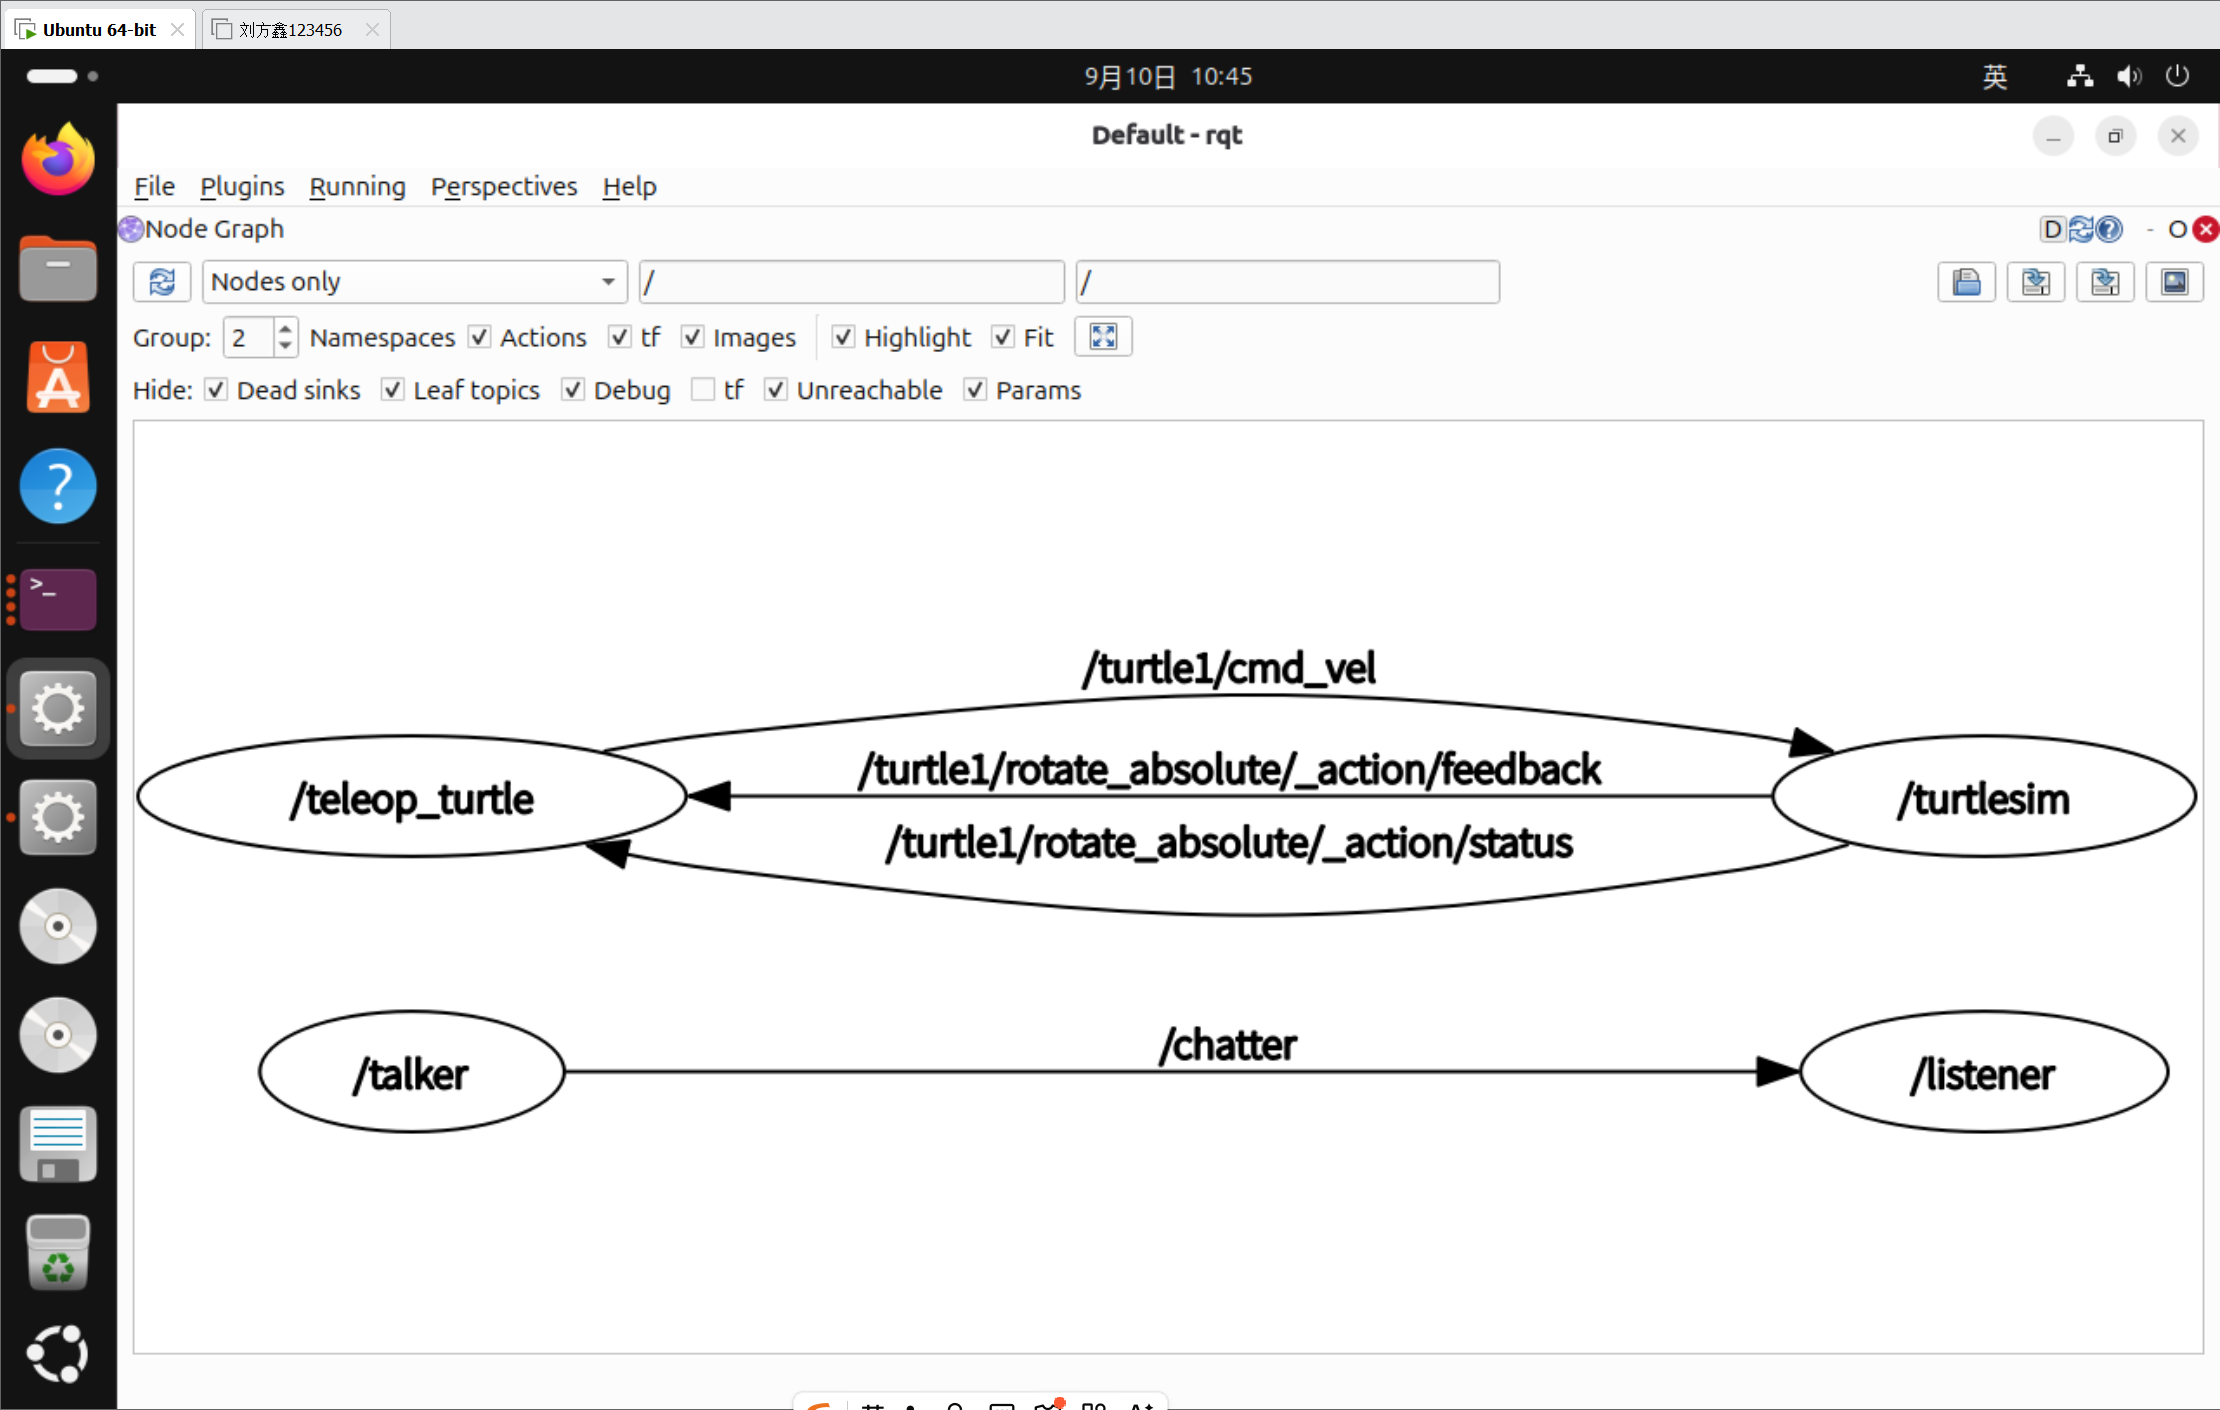
\includegraphics[width=0.8\textwidth]{Figure/RQT Node Graph 可视化.png}
  \caption{RQT Node Graph 可视化}
  \label{fig:RQT Node Graph 可视化}
\end{figure}

\section{ROS2系统架构}
前面两个小游戏你已经玩过了，节点能跑起来，rqt 里也能看到它们之间的连线。不过这些都还停留在“会用”的层面。这一节我们把 ROS2 拆开，从整体框架上看一看它到底由哪几层构成，以及为什么要这样分层。

\subsection{分层架构总览}
ROS2 的整体结构可以用一张“千层饼”式的图来描述，从上到下依次是：应用层、ROS2 客户端库、客户端库核心 rcl、中间件抽象层 RMW、DDS 实现层、操作系统层。相邻两层之间是双向的调用关系：上层向下层提出请求，下层把结果和事件回传给上层。

\begin{figure}[htbp]
\centering
\begin{tikzpicture}[font=\small,
  layer/.style={draw=black!65, rounded corners=2.5pt, minimum width=9.2cm,
                minimum height=1.05cm, align=center, text width=8.6cm, inner sep=3pt}]

\node[layer, fill=blue!10]  (app)  {应用层\\[-1pt]{\footnotesize 用户节点 · rqt · 命令行工具}};
\node[layer, fill=cyan!10,  below=4mm of app]  (rcl)  {ROS2 客户端库\\[-1pt]{\footnotesize rclpy · rclcpp · rcljava · rclnodejs · \dots}};
\node[layer, fill=teal!12,  below=4mm of rcl]  (rclc) {客户端库核心 rcl（C 语言实现）};
\node[layer, fill=orange!15,below=4mm of rclc] (rmw)  {中间件抽象层 RMW};
\node[layer, fill=red!10,   below=4mm of rmw]  (dds)  {DDS 实现层\\[-1pt]{\footnotesize Fast DDS · Cyclone DDS · Connext · \dots}};
\node[layer, fill=green!12, below=4mm of dds]  (os)   {操作系统层\\[-1pt]{\footnotesize Linux · Windows · macOS · 驱动与网络协议栈}};

\foreach \a/\b in {os/dds, dds/rmw, rmw/rclc, rclc/rcl, rcl/app}{
  \draw[<->, >=stealth, thick, black!55] (\a.north) -- (\b.south);
}

\draw[decorate, decoration={brace, amplitude=4pt, mirror}, black!60]
  ($(app.north east)+(0.35,0)$) -- ($(rclc.south east)+(0.35,0)$)
  node[midway, right=7pt, align=left, font=\footnotesize,
       text width=2.6cm] {ROS2 自身的实现，\\跨语言绑定};

\draw[decorate, decoration={brace, amplitude=4pt, mirror}, black!60]
  ($(rmw.north east)+(0.35,0)$) -- ($(rmw.south east)+(0.35,0)$)
  node[midway, right=7pt, align=left, font=\footnotesize,
       text width=2.6cm] {统一接口，\\屏蔽各家差异};

\draw[decorate, decoration={brace, amplitude=4pt, mirror}, black!60]
  ($(dds.north east)+(0.35,0)$) -- ($(dds.south east)+(0.35,0)$)
  node[midway, right=7pt, align=left, font=\footnotesize,
       text width=2.6cm] {第三方中间件，\\可自由替换};
\end{tikzpicture}
\caption{ROS2 的分层架构。自下而上依次是操作系统层、DDS 实现层、中间件抽象层 RMW、客户端库 RCL 以及最顶端的应用层，相邻两层之间为双向调用关系}
\label{fig:ROS2分层架构}
\end{figure}

图~\ref{fig:ROS2分层架构} 中两侧的括号标出了各层的归属：从应用层到客户端库核心 rcl，这三层是 ROS2 官方自己实现的；中间件抽象层 RMW 是统一接口；最下面的 DDS 实现层则来自第三方。接下来我们自下而上，一层一层地看。



\subsection{操作系统层}
这一层最好理解。ROS2 自己并不是一个操作系统，它只是跑在 Linux、Windows 或 macOS 之上的一个中间件框架。真正去驱动硬件、管理进程、收发底层网络数据包这些脏活累活，全部交给操作系统来完成。也正因为如此，ROS2 才能在这么多平台上跑起来：只要那个平台提供的系统调用和网络协议栈足够完整，上面的各层就可以原封不动地搬过去。

顺带说一句，我们在第一章里折腾 Ubuntu 虚拟机，其实就是在给上面的几层准备一块合适的“地基”。

\subsection{DDS 实现层}
想弄懂这一层，你得先回答两个问题：DDS 到底是什么？以及为什么 ROS2 里会同时存在好几套 DDS 实现？

\subsubsection{DDS 是什么}

DDS，全称 Data Distribution Service，中文叫“数据分发服务”，是由对象管理组 OMG（Object Management Group）在 2003 年发布、2007 年修订的一套分布式系统通信标准。

它的通信方式和 ROS 里的话题发布订阅几乎一模一样：一方把数据“发布”到某个主题上，关心这个主题的另一方“订阅”后就能收到，双方不需要事先知道对方是谁。除此之外，DDS 还提供了相当丰富的服务质量（QoS）策略，用来规定通信的可靠性、持久性、传输方式等要求。

正因为设计理念如此契合，ROS2 干脆不再自己另造一套通信协议，而是直接把 DDS 拿来当作底层的通信支柱。

\subsubsection{为什么会有多套 DDS 实现}

DDS 只是一份标准文档，标准本身不能运行，得有人照着它写出真正的程序，这些程序就叫“DDS 实现”。目前常见的实现有 eProsima 的 Fast DDS、Eclipse 的 Cyclone DDS、RTI 的 Connext DDS 等。它们遵守同一份标准，但侧重点各不相同：有的偏重性能，有的体积小巧，有的面向商用场景提供技术支持。

既然标准是统一的，那多准备几套实现就不会给上层添麻烦，想换随时换。至于这些差异是怎么被“抹平”的，就要看下面这一层了。

\subsection{中间件抽象层 RMW}
RMW 是 ROS Middleware 的缩写，也就是中间件抽象层。它的作用可以用一句话概括：\textbf{给上面一个统一的接口，把下面各家的差异藏起来}。

为什么不直接把 DDS 暴露给上层呢？因为直接用 DDS 其实挺麻烦的。创建一次通信要设置分区、主题名称、发现模式、消息类型等一大堆参数，还要记得在不用的时候逐项清理。这些琐碎而重复的配置如果让每个写节点的同学自己处理，代码会变得又臭又长。

于是 ROS2 在这中间加了一层 RMW：它定义好一套固定的接口，无论底下换成 Fast DDS 还是 Cyclone DDS，上层看到的 API 都完全一样。那些繁琐的配置也就顺理成章地在 RMW 和 RCL 里统一完成了。

\begin{lstlisting}[language=bash,title={查看与切换 DDS 实现}]
# 查看当前使用的 DDS 实现
ros2 doctor --report | grep middleware

# 通过环境变量切换（需要系统里已安装对应的 DDS）
export RMW_IMPLEMENTATION=rmw_cyclonedds_cpp
\end{lstlisting}

\subsection{客户端库 RCL 与语言绑定}
RCL 是 ROS Client Library 的缩写，也就是 ROS2 客户端库。它建立在 RMW 之上，把 ROS 里的节点、话题、服务、参数、Action 这些概念包装成一套好用的 API。

这里有个细节值得留意：RCL 的底层实现是用 C 语言写的，因为 C 是众多高级语言的“共同祖先”，基于它再去封装其它语言会轻松很多。所以官方的 rclpy（Python）和 rclcpp（C++）都是直接建立在这套 C 实现之上的。这也是为什么后面我们用两种语言写节点时，代码结构会如此相似。

社区还用同样的方式把 ROS2 搬到了更多语言和平台上，比如在 Android 应用或网页里也能和 ROS2 通信：

\begin{table}[htbp]
  \centering
  \caption{ROS2 的常见多语言客户端库}
  \label{tab:rcl-bindings}
  \small
  \begin{tabular}{@{}lll@{}}
    \toprule
    语言 & 客户端库 & 项目地址 \\
    \midrule
    Python & rclpy & \url{https://github.com/ros2/rclpy} \\
    C++ & rclcpp & \url{https://github.com/ros2/rclcpp} \\
    Java & rcljava & \url{https://github.com/esteve/ros2_java} \\
    Rust & rclrust & \url{https://github.com/ros2-rust/ros2_rust} \\
    Node.js & rclnodejs & \url{https://github.com/RobotWebTools/rclnodejs} \\
    Go & rclgo & \url{https://github.com/juaruipav/rclgo} \\
    Lua & rcllua & \url{https://github.com/jbbjarnason/rcllua} \\
    Kotlin & rclkin & \url{https://github.com/ros2java-alfred/ros2_kotlin} \\
    Swift & rclswift & \url{https://github.com/atyshka/ros2_swift} \\
    C\# & rclcs & \url{https://github.com/RobotecAI/ros2cs} \\
    \bottomrule
  \end{tabular}
\end{table}

\subsection{应用层}
最上面就是我们自己写代码、以及 rqt、命令行工具这些开发工具所在的层了。本书后面写的所有节点代码，其实都住在这里。它们不需要关心底下的通信是怎么实现的，只要调用客户端库提供的 API 就好，这也正是分层带来的好处。

\section{ROS2中间件DDS架构}
\subsection{中间件}
\subsubsection{中间件是什么}
中间件是一种独立的系统软件或服务程序，分布式应用软件借助这种软件在不同的技术之间共享资源。中间件位于客户机/ 服务器的操作系统之上，管理计算机资源和网络通讯。是连接两个独立应用程序或独立系统的软件。相连接的系统，即使它们具有不同的接口，但通过中间件相互之间仍能交换信息。执行中间件的一个关键途径是信息传递。通过中间件，应用程序可以工作于多平台或OS环境。\begin{figure}[h]
  \centering
  
\includegraphics[width=0.8\textwidth]{Figure/熊猫表情.jpg}
\end{figure}

这是在说什么，怎么一个字都听不懂（）




\ifcsname wholebook\endcsname
\expandafter\endinput
\fi

% 单独编译模式: 在顶层(无未闭合条件)执行 \end{document} 收尾。
\end{document}